\documentclass[
    a4paper,
    12pt,
    parskip=half,
    ngerman,
    bibliography=totoc,
    listof=totoc
]{scrartcl}

\usepackage[a4paper,margin=2.5cm]{geometry}
\usepackage{setspace}

\onehalfspacing

\usepackage[utf8]{inputenc}
\usepackage[T1]{fontenc}
\renewcommand{\familydefault}{\sfdefault} % Serifenlose Schrift
\usepackage[ngerman]{babel}
\usepackage[autostyle]{csquotes} % Anführungszeichen mit \enquote{text}

\usepackage{graphicx}
\graphicspath{{media/}}
\usepackage{wrapfig}    % Für von Schrift umflossene Bilder und Tabellen
\usepackage[font=small,labelfont=bf, indention=0pt, format=plain]{caption}
\usepackage{subcaption} % Subcaption bei mehreren Bildern in einer figure
\usepackage{tabularx}   % Tabellen
\usepackage{booktabs}   % Horizontale Linien für Tabellen
\usepackage{acro}       % Abkürzungen
\usepackage{amsmath}    % Mathematische Symbole
\usepackage{amssymb}    % \boxtimes Symbol im ai_discalaimer.tex

\usepackage{lipsum} % Lorem Ipsum-Generierung 

% Einbinden von Programmcode (Kommentar entfernen falls benötigt)
% \usepackage{xcolor}
% \usepackage{minted}
% \setminted{
%     frame=single,
%     framerule=0.8pt,
%     framesep=6pt,
%     rulecolor=\color{black},
%     breaklines=true,
%     fontsize=\small,
%     tabsize=2,
%     autogobble
% }

\usepackage[backend=biber,
    style=ieee,
    sorting=none,
    dashed=false
]{biblatex}
\addbibresource{literatur.bib}

\usepackage[hidelinks, colorlinks=true, urlcolor=blue, linkcolor=black, citecolor=black]{hyperref}

% ==================================================
%            BENUTZERDEFINIERTE BEFEHLE
% ==================================================

\newcommand{\Autor}{<Name einfügen>}
\newcommand{\Titel}{<Titel einfügen>}

% ==================================================
%                   ABKÜRZUNGEN
% ==================================================

% Quick Guide: https://www.namsu.de/Extra/pakete/Acro.html#:~:text=Abk%C3%BCrzungen%20und%20Akronyme%20aufrufen
% \DeclareAcronym{PDF}{short = PDF, long = Portable Document Format, long-plural = s}
\DeclareAcronym{PDF}{short = PDF, long = Portable Document Format, long-plural = s}


% ==================================================
%                  BEGINN DOKUMENT
% ==================================================

\hypersetup{pdftitle={\Titel}, pdfauthor={\Autor}, pdflang={de}}
\begin{document}

\pagenumbering{roman}

\begin{titlepage}
    % DB InfraGO + DHBW Mannheim Logos
    \begin{minipage}[t]{\textwidth}
        \begin{minipage}[c]{0.49\textwidth}
            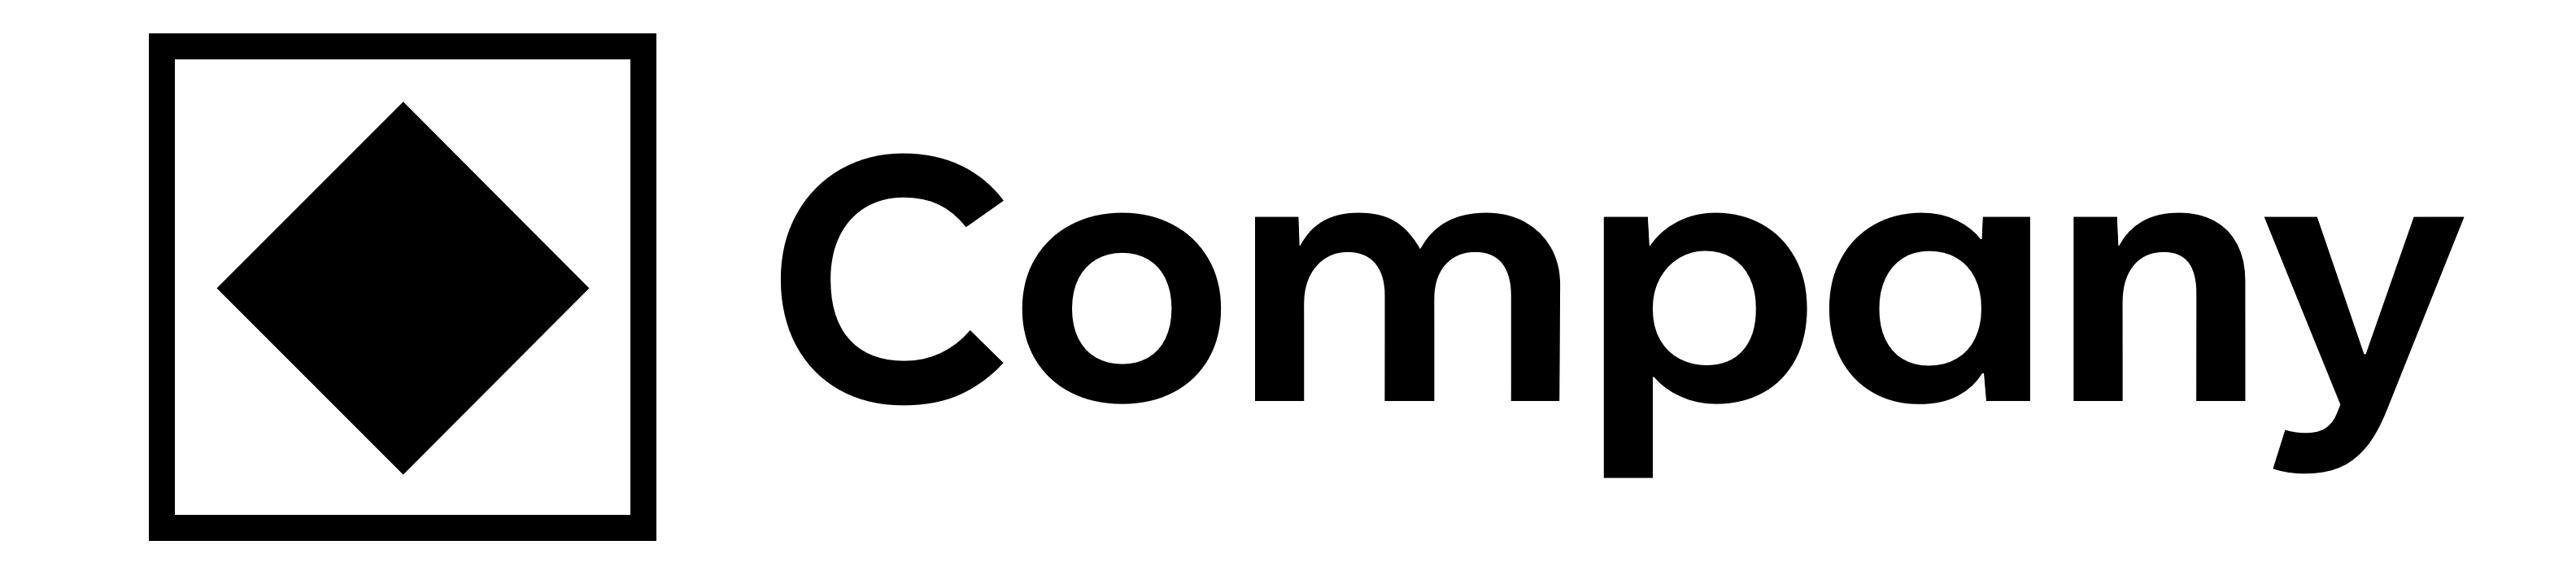
\includegraphics[width=0.8\textwidth]{Company_Logo.png}
        \end{minipage}
        \hfill
        \begin{minipage}[c]{0.49\textwidth}
            \hfill
            
\includegraphics{DHBW_MA_Logo.jpg}
        \end{minipage}
    \end{minipage}

    \vspace{1em}

    \begin{center}
        \huge{\Titel} \\[1.5cm]
        \textbf{\Large{Praxisarbeit / Studienarbeit / Bachelorarbeit}} \\[1.5cm]
        \large{des Studiengangs <Studiengang>} \\[0.5cm]
        \large{an der Dualen Hochschule Baden-Württemberg Mannheim} \\[1.5cm]
        \large{von} \\[0.5cm]
        \large{\Autor}

        \vfill

        \begin{minipage}{\textwidth}
            \begin{tabbing}
                Wissenschaftlicher Betreuer: \hspace{0.85cm}\=\kill

                Bearbeitungszeitraum: \> xx.xx.XXXX - xx.xx.XXXX \\[1.5mm]
                Matrikelnummer, Kurs: \> 1234123, TINFxxXXx \\[1.5mm]
                Dualer Partner: \> Company, Mannhheim \\[1.5mm]
                Betrieblicher Betreuer: \> Max von Mustermann \\[1.5mm]
                Wissenschaftlicher Betreuer \> Prof. Dr. Joe Doe
            \end{tabbing}
        \end{minipage}
    \end{center}
\end{titlepage}
\newpage

\section*{Sperrvermerk}

Die vorliegende Bachelorarbeit mit dem Titel \enquote{\Titel} beinhaltet interne und vertrauliche Informationen der DB InfraGO AG und unterliegt somit folgendem Sperrvermerk gemäß §20 Abs. (4) der DHBW StuPrO:

Der Inhalt dieser Arbeit darf weder als Ganzes noch in Auszügen Personen außerhalb des Prüfungsprozesses und des Evaluationsverfahrens zugänglich gemacht werden, sofern keine anderslautende Genehmigung des Dualen Partners vorliegt.\\[1.5cm]

% Die Sperrfrist läuft bis zum xx.xx.XXXX

\begin{minipage}{\textwidth}
    \begin{minipage}[t]{0.4\textwidth}
        \begin{center}
            \hrule
            \vspace{1.5mm}
            Ort, Datum
        \end{center}
    \end{minipage}
    \hfill
    \begin{minipage}[t]{0.4\textwidth}
        \begin{center}
            \hrule
            \vspace{1.5mm}
            Unterschrift
        \end{center}
    \end{minipage}
\end{minipage}
\newpage

\section*{Kurzfassung (Abstract)}

\subsection*{Kurzfassung (Deutsch)}
\lipsum[1]

\subsection*{Abstract (English)}
\lipsum[1]
\newpage

\section*{Ehrenwörtliche Erklärung}
Ich versichere hiermit, dass ich die vorliegende Arbeit mit dem Titel \enquote{\Titel} selbstständig verfasst und keine anderen als die angegebenen Quellen und Hilfsmittel benutzt habe. \\[1.5cm]

\begin{minipage}{\textwidth}
    \begin{minipage}[t]{0.4\textwidth}
        \begin{center}
            \hrule
            \vspace{1.5mm}
            Ort, Datum
        \end{center}
    \end{minipage}
    \hfill
    \begin{minipage}[t]{0.4\textwidth}
        \begin{center}
            \hrule
            \vspace{1.5mm}
            Unterschrift
        \end{center}
    \end{minipage}
\end{minipage}
\newpage

\section*{Erklärung zur Verwendung von KI-Systemen}

Der Autor erklärt, dass er

\begin{itemize}
    \item[$\boxtimes$] sich aktiv über die Leistungsfähigkeit und Beschränkungen der in dieser Arbeit eingesetzten KI-Systeme informiert hat;
    \item[$\boxtimes$] alle Inhalte aus wissenschaftlich anerkannten Quellen entnommen und entsprechend gekennzeichnet hat; alle Inhalte unter Anwendung wissenschaftlicher Methoden im Rahmen der vorliegenden Arbeit von ihm selbst entwickelt hat;
    \item[$\boxtimes$] sich bewusst ist, dass er als Autor dieser Arbeit die Verantwortung für die in ihr gemachten Angaben und Aussagen trägt.
\end{itemize}

Bei der Erstellung der Arbeit hat der Autor die folgenden auf künstlicher Intelligenz (KI) basierten Systeme in der im Folgenden dargestellten Weise benutzt:

\vspace{0.4em}

\begin{tabularx}{\textwidth}{p{0.36\textwidth}p{0.24\textwidth}X}
    \toprule
    \textbf{Arbeitsschritt} & \textbf{Eingesetze(s) KI-System(e)} & \textbf{Beschreibung der Verwendungsweise} \\
    \midrule
    Placeholder-Arbeitsschritt & Placeholder-KI & Placeholder-Beschreibung \\
    \addlinespace
    Literaturverwaltung und Zitationsmanagement & Placeholder-KI & Formatierung von BibTeX Quellenangaben \\
    \bottomrule
\end{tabularx}

\vspace{3em}

\noindent
\begin{minipage}[t] {0.48\textwidth}
    \rule{\linewidth}{0.5pt}
    Ort, Datum, Unterschrift
\end{minipage}
\newpage

\tableofcontents
\newpage

\printacronyms[name=Abkürzungsverzeichnis, heading=section*]
\newpage

\pagenumbering{arabic}

%        Einleitung
% =========================

\section{Einleitung}

\lipsum[1]

Beispiel einer Abkürzung: \ac{PDF}
\newpage

%        Hauptteil
% =========================
\section{Hauptteil}
\lipsum[1-8]

% Beispielzitate
\cite{muellermueller2024reinforcement}
\cite{schmidt2023einfuhrung}
\newpage


%           Fazit
% =========================

\input{fazit.tex}
\newpage

% ==================================================
%              ANFANG DER BIBLIOGRAPHIE
% ==================================================

\printbibliography
\newpage

\end{document}
